\section{Appendix}


\subsection{Composition operator for Solution}\label{def:compOperatorMu} 
Given $C= \{ C_1,..,C_n \}$ a set of LTSs, $L_c$ an LTS where $\Sigma = \Sigma_{C_1} \ \cup \ .. \ \cup \Sigma_{C_n}  \ \cup \ \Sigma_{L_c}$, we define a composition operator $||_{\mu}$ as $(C_1 || \ .. \ || \ C_n \ || \ L_c) \ \setminus \ \text{T}$, where $\text{T} = \{ ((c_1, .., c_n, lc), l, (c_1', .., c_n', lc')) \in \xrightarrow[]{}_{C_1||..||C_n||L_n} \ | \ l \notin f_{C_{i\in 0,..,n}}(c_{i \in 0,..,n}, d) \ \wedge \ d \in \xrightarrow[]{}_{L_N}(lc)  \}$ where $f_M: S \times \Sigma \xrightarrow[]{} \{ \Sigma \}$ is a function defined as $f_M(s, d) = \{ l \ | \ l \in \Sigma_u \ \vee \ (l\pi \ \text{where} \  \pi \ \text{is a controllable path to} \ s' \ \wedge \ s' \xrightarrow[]{d}_{M} ) \}$.

\subsection{Overview}

We show two compositions referred to in the Overview section. The first is the parallel composition of the original modular plant ($M_1\|M_2\|M_3$). The second is the composition of the plant where a subplant has been controlled and minimized ($M_3 \| (M_1 
            \| M_2)_{cont}$). Note the difference in size. 

\begin{figure}[h!]
    \centering
   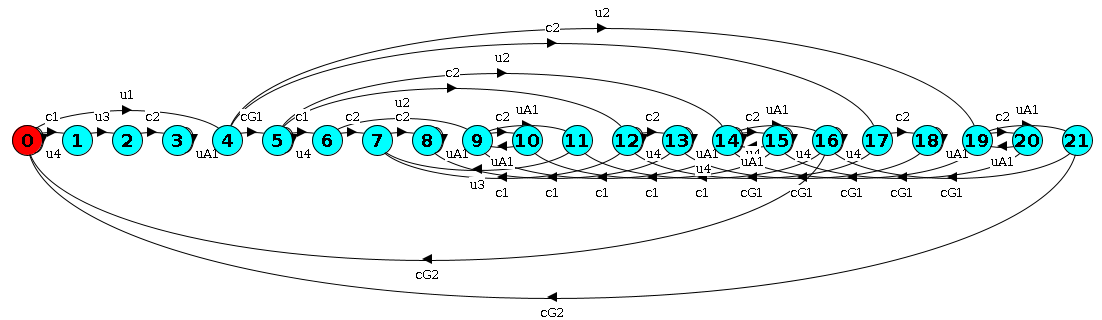
\includegraphics[width=1\linewidth]{sections/example_img/imgs/fig_M1_M2_M3.png}
    \caption{Composed plant  $M_1 \| M_2 \|  M_3$ that a monolithic synthesis approach 
    would 
    have to build to solve the control problem $\mathcal{E}$.} \label{fig:monolithic}
\end{figure}


\begin{figure}[h!]
          \centering
         % 
         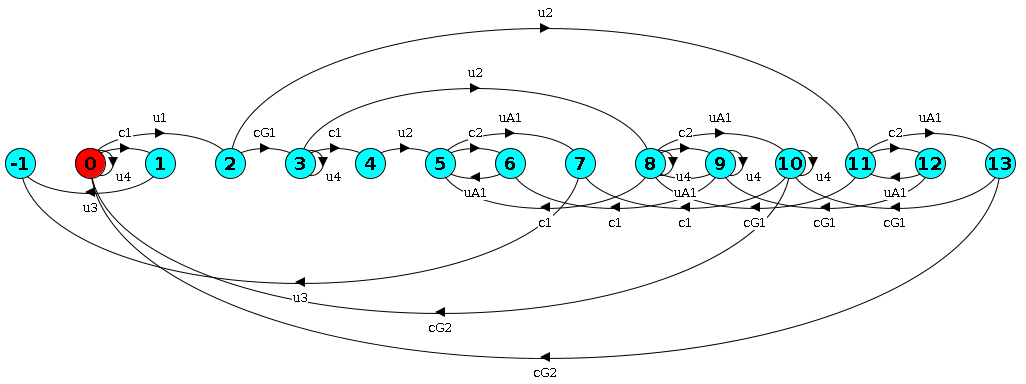
\includegraphics[width=\linewidth]{sections/example_img/imgs/fig_M3_safeass.png}
          \caption{Plant $M_3 \| (M_1 
            \| M_2)_{cont}$. It is nearly half the size of $M_1 \| M_2 
            \| M_3$
            }
          \label{fig:M3||SafeAss}
      \end{figure}

\newpage
% \subsection{Experimental Results}
% \noindent
% The following tables shows a performance comparison of the compositional synthesis approach referenced in Subsection \textbf{Results for DES Controller Synthesis via Reactive Synthesis}.
% ``Parse Error" refers to a crash of the Spectra parser. Spectra developers (personal communication) suspect that this is due to the size of the input file containing the  translated control problem.
% \begin{table}[h!]
% \centering
% \begin{tabular}{lccc}
% \toprule
% \textbf{Case} & \makecell{\textbf{Spectra Compositional}\\ \textbf{with Modular Translation}} & 
% \makecell{\textbf{Spectra Monolithic with}\\ \textbf{Non-Modular Translation}}
% & 
% \makecell{\textbf{Spectra Monolithic with}\\ \textbf{Modular Translation}} \\ 
% \midrule
% ATr-3-6  & 250s  & TO & 560s \\ 
% \hline
% AT!r-8-1 & 15s & TO & 1104s \\ 
% \hline
% BW-8-2 & 82s & TO & 7s \\ 
% \hline
% CM-2-5 & 8s & TO & 54s \\ 
% \hline
% RS-3-3   & 2s & 6.5s & 3.9s \\ 
% \hline
% TA-8-8 & 421s & OOM & 768s  \\ 
% \hline
% TL-3-6 & 88s & Parser Error & 310s \\
% \hline
% DP-8   & 29s & TO & 1181s \\ 
% \hline
% GR-11 & 37s & OOM & 29s \\  
% \hline
% MO-2 & 5s & 92s & 35s  \\  
% \hline
% PC-4 & 4.3s & OOM & 237s  \\  
% \bottomrule
% \end{tabular}
% \caption{Performance Comparison (Spectra focused)}
% \label{tab:spectra_comparison}
% \end{table}

% %
% %% Strix table
% %
% \begin{table}[h!]
% \centering
% \begin{tabular}{lcccc}
% \toprule
% \textbf{Case} & \makecell{\textbf{Strix Compositional}\\ \textbf{with Modular Translation}} & 
% \makecell{\textbf{Strix Monolithic with}\\ \textbf{Non-Modular Translation}}
% & 
% \makecell{\textbf{Strix Monolithic with}\\ \textbf{Modular Translation}} \\ 
% \midrule
% ATr-2-2   & 2.1s & 3.5s  & 44s \\ 
% \hline
% AT!r-2-1   & 1.1s & 1s  & 32s \\ 
% \hline
% BW-2-2   & 3.4s & 1s & 24s \\ 
% \hline
% CM-1-2   & 1.3s & 7s & 7s \\ 
% \hline
% RS-2-2    & 4.3s & 12s & 61s \\ 
% \hline
% TA-2-2   & 7.3s & 63s & 732s \\ 
% \hline
% TL-2-1   & 1.4s & 2s & 12s \\ 
% \hline
% DP-2     & 0.8s & 4s & 25s \\ 
% \hline
% GR-2   & 42s & OOM  & 326s \\  
% \hline
% MO-2 & 1233s & OOM  & TO  \\  
% \hline
% PC-4   & 37s & 43s & 322s \\
% \bottomrule
% \end{tabular}
% \hspace{0.1 cm}
% \caption{Performance Comparison (Strix Focused)}
% \label{tab:strix_comparison}
% \end{table}



%% Theorem proofs.
\newpage
\subsection{Theorem \ref{lemma:non-flooding-equivalence}}
This Lemma will be used in the proof of Theorem \ref{lemma:non-flooding-equivalence}.
\begin{lemma}
    \label{lemma:selfloop-traces-mu}
    Given a LTS $M$ and $M' = M / \! \sim_\Upsilon$, if there is a trace $\pi \in tr(M')$ and $s\in S_{M'}$ such that $\pi \in \Upsilon^*$ and $s \xrightarrow[]{\pi}_{M'} s$ then $\forall l \in \pi$ we have $s \xrightarrow[]{l}_{M'} s $ 
\end{lemma}
\textbf{Proof.}
We prove by contradiction. Suppose a trace $\pi \in tr(M')$ and $s\in S_{M'}$ such that $\pi \in \Upsilon^*$, $s \xrightarrow[]{\pi}_{M'} s$, and $\exists l \in \pi$ such that $(s, l, s) \notin \xrightarrow[]{}_{M'}$.
Without loss of generality can assume that $\pi = l \pi'$ and $\exists s' \in S_{M'} \cdot s\neq s'$ such that  $s\xrightarrow[]{l}_{M'} \!s'$, $s'\xrightarrow[]{\pi'}_{M'} \!s$. 
Because $s \neq s'$ and $M'$ is minimized respect to $\sim_{\Upsilon}$ we have that $s$ and $s'$ are not equivalent.  However, by Def.~\ref{def:synth-equiv} we have that $s$ and $s'$ are, reaching a contradiction: State $s$ can simulate $s'$ by first going though $l$, and state $s'$ can simulate $s$ by going through $\pi'$.
$\hfill \square$
\\
\\
\noindent The following theorem proves that  a control problem with a formula  of the form $\square \Diamond (\bigwedge_{l \in (\mu \cup \mu')} \neg l) \implies \varphi$ where $\varphi$ is  GR(1)  can be solved as a GR(1) control problem. We use notation $\mathcal{M} \setminus T$ where $\mathcal{M}$ is an LTS and $T$ is a set of transitions over $\mathcal{M}$ to denote the result of removing each transition in $T$ from $\mathcal{M}$. 

\vspace{0.2cm}
\textbf{Theorem \ref{lemma:non-flooding-equivalence}} 
Given a control problem $\mathcal{E} =  \langle \mathcal{M'} \setminus \{ (s, l, s) \ | \ l \in \mu \cup \mu' \}, \Sigma_c, \varphi \rangle$ and $\mathcal{E'} =  \langle \mathcal{M'}, \Sigma_c, 
     \square \Diamond (\bigwedge_{l \in (\mu \cup \mu')} \neg l)$ $\implies \varphi \rangle$ where $\mathcal{M'} = \mathcal{M} \setminus \{ M_{sub} \} \cup \{ M_{cont} \slash \! \sim_\Upsilon \}$, $\Sigma_c \subseteq \Sigma$ is a set of controllable events, $\mu \ \text{and} \ \mu'$ are sets of events and $M_{cont}$ is a controlled subplant for $\langle \mathcal{M}_{sub}, \Sigma_c, \square \Diamond (\bigwedge_{l \in \mu} \neg l) \implies \varphi\rangle$ where $\mathcal{
     M}_{sub} \subseteq \mathcal{M}$. If there is a solution $C = (S_c, \Sigma, \xrightarrow[]{}_{c}, \hat{s}_c)$ for control problem $\mathcal{E}$, then $C'$ is a solution for $\mathcal{E'}$ where $C' = (S_{c'}, \Sigma, \xrightarrow[]{}_{c'}, \hat{s}_c)$ is defined as follows:
     \begin{itemize}
         \item $S_{C'} = S_C$
         \item $\xrightarrow[]{}_{C'} =  \xrightarrow[]{}_{C} \cup \ \{ (s, l, s) \ | \ s \in S_c \ \wedge \ l \in \Sigma_u \cap (\mu \cup \mu') \ \wedge \ \exists (s_{\mathcal{M'}}, s_{c}) \in S_{\mathcal{M'}||C} \ \cdot \ (\hat{s_{\mathcal{M'}}}, \hat{s_{C}}) \xrightarrow[]{}_{\mathcal{M'}\|C} (s_{\mathcal{M'}}, s_{C}) \ \wedge \ (s_{\mathcal{M'}}, l, s_{\mathcal{M'}}) \in \xrightarrow[]{}_{\mathcal{M'}} \}$. 
     \end{itemize}
     Also, if there is no solution for $\mathcal{E}$ then there is no solution for $\mathcal{E}'$.
\\ \\
\textbf{Proof.} We  prove first that if there exists such solution $C$ for $\mathcal{E}$, then $C'$ is a solution for $\mathcal{E'}$:
\begin{itemize}
    %%% Legality
    \item $C'$ is legal for $\mathcal{M'}$ with respect to $\Sigma_u = \Sigma \setminus \Sigma_c$ \\
    The proof is by contradiction. Suppose that $C'$ is not legal for $\mathcal{M'}$ with respect to $\Sigma_u$. Therefore exists $(s_{C'},s_{\mathcal{M'}})\in S_{C'||\mathcal{M'}}$ and $l \in \Sigma_u$ such that $l \in \xrightarrow[]{}_{\mathcal{M'}}\!(s_{\mathcal{M'}})$ and $l \notin \xrightarrow[]{}_{C'}\!(s_{C'})$. In addition, there is also a trace $\pi \in tr(C') \ \cdot \ \hat{s_{C'}} \xrightarrow[]{\pi} s_{C'}$. Trace $\pi$ may not be in $tr(C)$, however we can build a trace $\pi' \in tr(C)$ that reaches the same state by removing any self loops labeled with $\ l \in \mu \cup \mu'$. This leads us to a contradiction because we assumed that $C$ was legal for $\mathcal{M'} \setminus \{ (s, l, s) \ | \ l \in \mu \cup \mu' \}$ with respect to $\Sigma_u$.
    
    %%% Deadlock-free
    \item $C' || \mathcal{M'}$ is deadlock-free \\ 
     Proven by contradiction. Suppose that $C' || \mathcal{M'}$ is not deadlock-free, so there is a deadlock state $s_d \in S_{C'||\mathcal{M'}}$ and a trace $\pi \in tr(C'||\mathcal{M'})$ such that $(\hat{s_{C'}},\hat{s_{\mathcal{M'}}}) \xrightarrow[]{}_{C'||\mathcal{M'}} s_d$. There are two options:
    \begin{itemize}
        \item $\pi \in tr(C)$ \\
        As we know that $C||\mathcal{M'}$ is deadlock-free, this trivially leads us to a contradiction coming from assumption that $C'||\mathcal{M'}$ is not deadlock free.
        %for the case that $\pi \in tr(C)$.
        \item $\pi \notin tr(C)$ \\
        If $\pi \notin tr(C)$ there exists a prefix $\pi'l$ of  $\pi$ such that $\pi' \in tr(C) \ \wedge \ \pi'l \notin tr(C)$, and there is a state $\bar{s_C} \in S_C$ such that $\hat{s_C} \xrightarrow[]{}_C \bar{s_C}$. By definition of $\xrightarrow[]{}_{C'}$, $l$ must be a self-loop transition and does not lead to a deadlock state, so this contradicts also initial assumption that $C'||\mathcal{M'}$ is not deadlock-free.
        %for the case that $\pi \notin tr(C)$.
        
        % As we know that $\xrightarrow[]{}_C \subseteq \xrightarrow[]{}_{C'}$, there is a transition 
        
        % and $S_C = S_{C'}$
        
        % $C||\mathcal{M'}$ is deadlock-free, this trivially lead us to a contradiction coming from assumption that $C'||\mathcal{M'}$ is not deadlock free and $\pi \in tr(C)$.
    \end{itemize}
    % As $S_{c} = S_{c'}$ and $\xrightarrow[]{}_{c} \ \subseteq \ \xrightarrow[]{}_{c'}$, there is a trace $\pi \in tr(C)$ such that $\hat{s}_c$


    
    %%% Formula satisf.
    \item $\forall \pi \in C' || \mathcal{M'},  \pi \vDash \square \Diamond (\bigwedge_{l \in (\mu \cup \mu')} \neg l) \implies \varphi $ \\
    It will be proven by contradiction. Suppose that $\exists \bar{\pi} \in tr( C' || \mathcal{M'}) \ \cdot \ \bar{\pi} \nvDash \square \Diamond (\bigwedge_{l \in (\mu \cup \mu')} \neg l) \implies \varphi$. There are two options:
    
    \begin{itemize}
        \item $\bar{\pi} \in tr(C)$ \\
        As we assume that $\bar{\pi} \nvDash \square \Diamond (\bigwedge_{l \in (\mu \cup \mu')} \neg l) \implies \varphi$, it holds that $\bar{\pi} \nvDash \varphi$. Also we know that $\bar{\pi} \in tr(C)$, so it holds that $\bar{\pi} \vDash \varphi$ because $C$ is solution for $\mathcal{E}$. This result lead us to a contradiction which comes from assuming that exists $\bar{\pi}$.
        \item $\bar{\pi} \notin tr(C)$ \\
        We assume that $\bar{\pi} \nvDash \square \Diamond (\bigwedge_{l \in (\mu \cup \mu')} \neg l) \implies \varphi$, so it holds that $\bar{\pi} \vDash \square \Diamond (\bigwedge_{l \in (\mu \cup \mu')} \neg l) \ \wedge \ \bar{\pi} \nvDash \varphi$. We can build a trace $\bar{\pi}' \subseteq \bar{\pi}$ such that $\bar{\pi}\in tr(C)$ if we remove occurrences of events $l\in \mu\cup\mu'$ of $\bar{\pi}$. As the formula  is stutter-free and there is no formula event present in $\mu\cup\mu'$, we conclude that $\bar{\pi}' \nvDash \varphi$ reaching a contradiction because $\bar{\pi'} \in tr(C)$ and $C$ is a solution for $\mathcal{E}$.
    \end{itemize}
Therefore, it is proven that $\forall \pi \in C' || \mathcal{M'},  \pi \vDash \square \Diamond (\bigwedge_{l \in (\mu \cup \mu')} \neg l) \implies \varphi$.
\end{itemize}
\noindent
What remains is to prove that if there is no solution $C$ for $\mathcal{E}$, then there is none for $\mathcal{E'}$ either. \\
It will be proven by counter reciprocal. I will prove that, if exists a solution $C'$ for $\mathcal{E'}$, then $C$ is a solution for $\mathcal{E}$. 
\begin{itemize}
    % legal
    \item $C$ is legal for $\mathcal{M'}\setminus \{ (s, l, s) \ | \ l \in \mu \cup \mu' \}$ with respect to $\Sigma_u = \Sigma \setminus \Sigma_c$. \\ 
    The proof is by contradiction. Suppose that $C$ is not legal for $\mathcal{M'} \setminus \{ (s, l, s) \ | \ l \in \mu \cup \mu' \}$ with respect to $\Sigma_u$. Therefore exists $(s_{C},s_{\mathcal{M'}})\in S_{C||\mathcal{M'}}$ and $l \in \Sigma_u$ such that $l \in \xrightarrow[]{}_{\mathcal{M'}}\!(s_{\mathcal{M'}})$ and $l \notin \xrightarrow[]{}_{C}\!(s_{C})$. In addition, there is also a trace $\pi \in tr(C) \ \cdot \ \hat{s_{C}} \xrightarrow[]{\pi}_{C||\mathcal{M'}} s_{C}$. As we know that $tr(C) \subseteq tr(C')$, we conclude that we can reach the same state leading us to a contradiction because we start assuming that $C'$ is legal for $\mathcal{M'}$ with respect to $\Sigma_u$.

    %deadlock-free
    \item $C||\mathcal{M'}$ is deadlock-free\\ 
    Proven by contradiction. Suppose that $C || \mathcal{M'}$ is not deadlock-free, so there is a deadlock state $s_d \in S_{C||\mathcal{M'}}$ and a trace $\pi \in tr(C||\mathcal{M'})$ such that $(\hat{s_{C}},\hat{s_{\mathcal{M'}}}) \xrightarrow[]{}_{C||\mathcal{M'}} s_d$. As we know that $tr(C) \subseteq tr(C')$, then $\pi \in tr(C'||\mathcal{M'})$. On the other hand, we know that $C'||\mathcal{M'} \setminus \{ (s, l, s) \ | \ l \in \mu \cup \mu' \}$ is deadlock-free and this trivially lead us to a contradiction coming from assumption that $C || \mathcal{M'}$ is not deadlock-free.

    % formula sat
    \item $\forall \pi \in C || \mathcal{M'} \setminus \{ (s, l, s) \ | \ l \in \mu \cup \mu' \},  \pi \vDash \varphi $ \\
    It will be proven by contradiction. Suppose that $\exists \bar{\pi} \in tr(C||\mathcal{M'} \setminus \{ (s, l, s) \ | \ l \in \mu \cup \mu' \}) \ \cdot \ \bar{\pi} \nvDash \varphi$. As $\bar{\pi} \in tr(\mathcal{M'} \setminus \{ (s, l, s) \ | \ l \in \mu \cup \mu' \})$, it holds trivially that $\bar{\pi} \vDash \square \Diamond (\bigwedge_{l \in (\mu \cup \mu')} \neg l)$. As we assume that $\bar{\pi} \nvDash  \varphi$, then it holds that $\bar{\pi} \nvDash \square \Diamond (\bigwedge_{l \in (\mu \cup \mu')} \neg l) \implies \varphi$.
    On the other hand, we know that $\bar{\pi}\in tr(C')$ (because $tr(C) \subseteq tr(C')$). This lead us to a contradiction because $C'$ is a solution for $\mathcal{E'}$, the contradiction comes from assuming that exists $\bar{\pi}$.
\end{itemize}
$\hfill \square$

\newpage
\subsection{Theorem \ref{lemma:traces-inclusion} }
\noindent Lemmas \ref{lemma:controller-equivalence} and \ref{lemma:traces-inclusion} will be used in the proof of Theorem \ref{PS+SOE_control}.
\begin{lemma}
    \label{lemma:controller-equivalence}
    Given a control problem $\mathcal{E} =  \langle \mathcal{M}, \Sigma_c, \varphi \rangle$, $\mathcal{M} = \{M_1, .., M_n\}$ and $M_{1}^{safe}$ is a Safe Controller for $\mathcal{E'} = \langle M_1, \Sigma_c \cup (\Sigma \setminus \Sigma_{M_1}), \varphi' \rangle$ where $\varphi'$ is a projected formula for $\Sigma_{M_1}$. If $C_M$ is a solution $\mathcal{E}$, then $C_M$ is a solution for $\mathcal{E'}$. 
\end{lemma}
\textbf{Proof.} \\
\begin{itemize}
    % legal
    \item $C_M$ is legal for $M_1$ with respect to $\Sigma_{u}' = \Sigma \setminus (\Sigma_c \cup (\Sigma \setminus \Sigma_{M_1}))$ \\
    The proof is by contradiction. Suppose that $C_M$ is not legal for $M_1$ with respect to $\Sigma_u' = \Sigma \setminus (\Sigma_c \cup (\Sigma \setminus \Sigma_{M_1}))$. Therefore exists $(s_{C_M}, s_{M_1}) \in S_{C_M||M_1}$ and $l \in \Sigma_u'$ such that $l \in \xrightarrow[]{}_{M_1}(s_{M_1})$ and $l \notin \xrightarrow[]{}_{C_M}(s_{C_M})$. In addition, there is also a trace $\pi \in tr(C_M || M_1)$ such that $(\hat{s_C}, \hat{s_{M_1}}) \xrightarrow[]{\pi}_{C_M||M_1} (s_{C_M},s_{M_1})$. \\
    As we know that $\pi \in tr(C_M)$, we can assume that $\pi \in tr(\mathcal{M})$ and $(\hat{s_C}, \hat{s_{\mathcal{M}}}) \xrightarrow[]{\pi}_{C_M||\mathcal{M}} (s_{C_M}, s_{\mathcal{M}})$ where $l \in \xrightarrow[]{}_{\mathcal{M}}(s_{\mathcal{M}})$ and $l \notin \xrightarrow[]{}_{C_M}(s_{C_M})$. This lead us to a contradiction because $\Sigma_u' \subseteq \Sigma_u$ and $C_M$ is a solution for $\mathcal{E}$, the contradiction comes from assuming that $C_M$ is not legal for $M_1$ with respect to $\Sigma_u' = \Sigma \setminus (\Sigma_c \cup (\Sigma \setminus \Sigma_{M_1}))$. \\
    
    % deadlock-free
    \item $C_M || M_1$ is deadlock-free \\
    The proof is by contradiction. Suppose that $C_M||M_1$ is not deadlock-free, so there is a deadlock state $s_d \in S_{C_M||M_1}$ and a trace $\pi \in tr(C_M||M_1)$ such that $(\hat{s_{C_M}}, \hat{s_{M_1}}) \xrightarrow[]{\pi}_{C_M||M_1} s_d$. As we know that $tr(C_M||M_1) \subseteq tr(C_M||\mathcal{M})$, then $\pi \in tr(C_M||\mathcal{M})$ and this trivially lead us to a contradiction because $C_M$ is a solution for $\mathcal{E}$, the contradiction comes from assuming that $C_M ||M_1$ is not deadlock-free. \\
    
    % formula sat
    \item $\forall \pi \in C_M || M_1$, $\pi \vDash \varphi'$ \\
    The proof is by contradiction. Suppose that $\exists \bar{\pi} \in tr(C_M||M_1) \ \cdot \ \bar{\pi} \nvDash \varphi'$. As we know that $tr(C_M||M_1) \subseteq tr(C_M||\mathcal{M})$, then $\pi \in tr(C_M || \mathcal{M})$. This lead us to a contradiction because $\varphi \xrightarrow[]{} \varphi'$, so as $C_M$ is a solution for $\mathcal{E}$, then $C_M$ should satisfy $\varphi'$. The contradiction comes from assuming that $\exists \bar{\pi} \in tr(C_M||M_1) \ \cdot \ \bar{\pi} \nvDash \varphi'$. 
    
    
\end{itemize}

$\hfill \square$

\begin{lemma}
    \label{lemma:traces-inclusion}
    Given a control problem $\mathcal{E} =  \langle \mathcal{M}, \Sigma_c, \varphi \rangle$, $\mathcal{M} = \{M_1, .., M_n\}$ and $M_{1}^{safe}$ is a Safe Controller for $\mathcal{E'} = \langle M_1, \Sigma_c \cup (\Sigma \setminus \Sigma_{M_1}), \varphi' \rangle$ where $\varphi'$ is a projected formula for $\Sigma_{M_1}$. If $C_M$ is a solution for $\mathcal{E}$, then $P_{\Sigma_{M_{1}}}(tr(C_M)) \subseteq tr(M_{1}^{safe})$. 
\end{lemma}
\textbf{Proof.}
The proof is by contradiction. Suppose that $\exists \pi \in tr(C_M)$ such that $P_{\Sigma_{M_{1}}}(\pi) \notin tr(M_{1}^{safe})$. As $C_M$ is a solution for $\mathcal{E}$, we know that $\pi \vDash \varphi$. Also, as $\varphi \xrightarrow[]{} \varphi'$, it holds that $\pi \vDash \varphi'$. Assuming that $P_{\Sigma_{M_{1}}}(\pi) \notin tr(M_{1}^{safe})$, by definition of safe controller we know that $\exists \ l\in \pi, s \in S_{M_1}$ such that $s \xrightarrow[]{l} s_e$ where $s_e$ is not a winning state (i.e., there is no controller that includes $s_e$). However, by Lemma \ref{lemma:controller-equivalence} we know that $C_M$ is a solution for $\mathcal{E'}$ and $\pi \in tr(C_M)$. This lead us to a contradiction because $P_{\Sigma_{M_{1}}}(tr(C_M))$ goes through winning states of $M_1$, so it must be contained in $tr(M_{1}^{safe})$. The contradiction comes from assuming that $\exists \pi \in tr(C_M)$ such that $P_{\Sigma_{M_{1}}}(\pi) \notin tr(M_{1}^{safe})$.\\
% Since $C_M$ is a solution for control problem $\mathcal{E}$, then $\forall \pi \in tr(C_M)$ it holds that $\pi \vDash \varphi$ and $P_{\Sigma_{M_{1}^{safe}}}(\pi)$ is a trace in $M_1$. This follows by using that $C_M \ || \ \mathcal{M}$ (and particularly $C_M \ || \ M_1$) is legal and deadlock-free and using that $\Sigma_{M_{1}^{safe}} = \Sigma_{M_{1}}$. \\
% By definition, we know that $\pi$ goes through winning states of $M_1$ for $\varphi$. Also, we know that $tr(M_{1}^{safe})$ goes through winning states of $M_1$ for $\varphi'$ GR(1) formula. \\ 
% As we know that $\varphi \xrightarrow[]{} \varphi'$, we can say also that $\pi$ goes through winning states of $M_1$ for $\varphi'$ GR(1) formula and that is definition for $tr(M_1^{safe})$. \\
% Then, $P_{\Sigma_{M_{1}^{safe}}}(tr(C_M)) \subseteq tr(M_{1}^{safe})$. \hfill $\square$

\noindent
The following theorem proves the equirealizability of the most important step that compositional synthesis uses. 

\textbf{Theorem \ref{PS+SOE_control}}  \\
    Given a synthesis tuple $(\mathcal{M}, \mathcal{C}, \mu)$, an LTL formula $\varphi$, and a set $\Sigma_c$ of controllable events.
    
    Let $M \subseteq \mathcal{M}$ with alphabet $\Sigma_{M} = \Upsilon \dot{\cup} \Omega$ where $\Upsilon$ has the events not shared with any other LTS in $\mathcal{M}\setminus M$ nor in $\varphi$. Let $\varphi'$ be a projection of $\varphi$ to $\Sigma_{M}$. 


   
    Let $M_{safe}$ be a safe controller for $\langle M, \Sigma_c, \Box\Diamond\bigwedge_{l\in \mu}\neg l \implies \varphi \rangle$.  
    Let $M_{cont}$ be the subplant $M$ controlled by $M_{safe}$ with shared events $\Omega$.

    If $M_{cont} \slash \! \sim_\Upsilon$ is deterministic and $\mu'$ is the set of self-looping events induced by $\sim_\Upsilon$ reduction, then  $(\mathcal{M}, \mathcal{C}, \mu) \cong_{\Sigma_c, \varphi} (\mathcal{M} \setminus \{M\} \cup \{M_{cont} \slash \! \sim_\Upsilon\}, \mathcal{C} \cup \{ M_{safe} \}, \mu \cup \mu')$.  \\ \\ 
\textbf{Proof.} 
We will use the notation $\mathcal{M'} = \mathcal{M} \setminus \{M\} \cup \{M_{cont} \slash \! \sim_\Upsilon\}$, $T = (\mathcal{M}, \mathcal{C}, \mu)$, $T' = (\mathcal{M} \setminus \{M\} \cup \{M_{cont} \slash \! \sim_\Upsilon\}, \mathcal{C} \cup \{ M_{safe} \}, \mu \cup \mu')$ as syntactic replacement. \\ \\
\textbf{$\xrightarrow{}$)} Given $S \in Cont_{\Sigma_c, \varphi}(T)$, we prove that $S \in Cont_{\Sigma_c, \varphi}(T')$. \\
This will be proven by existence of $\hat{C_{M}}$ such that is a solution for $\mathcal{E'} = \langle \mathcal{M'}, \Sigma_c, \square \Diamond \bigwedge_{l \in \mu \cup \mu'} \neg l \implies \varphi \rangle$ and $\hat{C_{M}} || M_{safe} || C = S$. \\
Since $S = C || C_M$ by definition where $C_M$ is a solution for $\mathcal{E} = \langle M, \Sigma_c, \square \Diamond \bigwedge_{l \in \mu} \neg l \implies \varphi \rangle$. We  demonstrate $\hat{C_M}$ exists using $\hat{C_M} = C_M$ and proving that:
\begin{enumerate}
    \item $C_M$ is a solution for $\mathcal{E'}$.
    \begin{enumerate}
        \item \textit{(formula satisfiability)} We  prove that 
        $\forall \pi \in (C_M || \mathcal{M'}) \ . \ \pi \vDash \square \Diamond \bigwedge_{l \in \mu \cup \mu'} \neg l \implies \varphi$ by contradiction. Suppose $C_M$ is not a solution for $\mathcal{E'}$ and there is a trace $\pi \in tr(C_M || \mathcal{M'})$ such that $\pi \nvDash 
        \square \Diamond \bigwedge_{l \in \mu \cup \mu'} \neg l \implies \varphi$. Also, it holds that $\pi \in C_M$.\\
        Since $C_M$ is a solution for $\mathcal{E}$, then $\forall \pi \in tr(C_M || \mathcal{M}) \ . \ \pi \vDash \square \Diamond \bigwedge_{l \in \mu} \neg l \implies \varphi$. \\
        Note that any trace $\pi$ that $\pi \vDash \square \Diamond \bigwedge_{l \in \mu} \neg l \implies \varphi$, it holds that \\ $\pi \vDash \square \Diamond \bigwedge_{l \in \mu \cup \mu'} \neg l  \implies \varphi$ because you are strengthening the assumption. Then, $\forall \pi \in tr(C_M) \ . \ \pi \vDash \square \Diamond \bigwedge_{l \in \mu \cup \mu'} \neg l \implies \varphi$ which contradicts the original assumption. \\
        Then, $\forall \pi \in (C_M || \mathcal{M'}) \ . \ \pi \vDash \square \Diamond \bigwedge_{l \in \mu \cup \mu'} \neg l \implies \varphi$.
        
        \item $C_M$ is legal for $\mathcal{M'}$ with respect to $\Sigma_u \cup (\mu \cup \mu')$.

         Proven by contradiction. \\
        Suppose $C_M$ is not legal for $\mathcal{M'}$ with respect to $\Sigma_u \cup (\mu \cup \mu')$. Then, $\exists \pi \in tr(C_M)$ such that $\exists l \in (\Sigma_u \cup (\mu \cup \mu')) \wedge \pi l \in tr(\mathcal{M'}) \wedge \pi l \notin tr(C_M)$. \\
        I separate into two cases: $l \in \Sigma_u \cup \mu$ or $l \in \mu'$
        \begin{enumerate}
            \item $l \in \Sigma_u \cup \mu$ \\
            This is not possible since $C_M$ is legal for $\mathcal{M}$ with respect to $\Sigma_u \cup \mu$ and $tr(\mathcal{M}) \subseteq tr(\mathcal{M'})$.
            \item $l \in \mu'$ \\
            By Lemma \ref{lemma:traces-inclusion}, if $\pi l \notin P_{M_{safe}}(tr(C_M))$, then $\pi l \notin tr(M_{safe})$. \\
            Then, by construction, $\pi \notin tr(M_1).$ \\
            Then, because $tr(\mathcal{M}) \subseteq tr(\mathcal{M'})$, $\pi l \notin tr(\mathcal{M'}).$ \\
            Which enter in contradiction with original assumption. Then, $C_M$ is legal for $\mathcal{M'}$ with respect to $\Sigma_u \cup (\mu \cup \mu')$.
        \end{enumerate}
        % Since $C_M$ is legal for $M$ with respect to $\Sigma_u \cup \mu$, for each $l \in (\Sigma_u \cup \mu)$ it holds that $\forall \pi \in tr(M) \ . \ \pi l \in tr(M) \ \text{implies} \ \pi l \in tr(C_M)$.  \\
        % By construction, it holds that $tr(M) \subseteq tr(\mathcal{M'})$. \\
        % Then, it holds that
        
        
        
        
        % $\forall l \in (\Sigma_u \cup \mu) \ . \ ()  
        
        % \wedge \pi l \in tr(\mathcal{M'}) \wedge \pi l \notin tr(C_M)$



        

        \item ($C_M || \mathcal{M'})$ is deadlock-free. \\
        Proven by contradiction. \\ 
        We suppose that $C_M || \mathcal{M'}$ has a deadlock state $(c, \mathcal{M'})$ reachable from initial state by a trace $\pi$. 
        Since $C_M || \mathcal{M}$ is deadlock free, there exists a label $l \in \Sigma_\mathcal{M}$ which is enabled in $(c, m)$, where $(c,m) \in S_\mathcal{M}$ is an state reachable by trace $\pi$.  
        Since $tr(\mathcal{M}) \subseteq tr(\mathcal{M'})$, it is not possible that $(c, m)$ has an enabled event which is disabled in $(c, \mathcal{M'})$. \\
        Then, ($C_M || \mathcal{M'})$ is deadlock-free.
        
    \end{enumerate}
    Then, $C_M$ is a valid solution for $\mathcal{E'}$. \\
    
    \item $C_M || M_{safe} || C = S$ \\
    This is correct iff $C_M || M_{cont} = C_M$ and it is correct because $tr(C_M |_{\Sigma_{M_{cont}}}) \subseteq tr(M_{cont})$, which is true by Lemma \ref{lemma:traces-inclusion}.
\end{enumerate}

\textbf{$\xleftarrow[]{}$)} Given $S \in Cont_{\Sigma_u, \varphi}(T')$, We prove that $S \in Cont_{\Sigma_u, \varphi}(T)$  by existence of $C_{M}$ such that is a solution for $\mathcal{E} = \langle \mathcal{M}, \Sigma_c, \square \Diamond \bigwedge_{l \in \mu} \neg l \implies \varphi \rangle$ and $C_M || C = S$. Since $S = \hat{C_M} || C || M_{safe}$ where $\hat{C_M}$ is a solution for  $\mathcal{E'} = \langle \mathcal{M'}, \Sigma_c, \square \Diamond \bigwedge_{l \in \mu \cup \mu'} \neg l \implies \varphi \rangle$.
We demonstrate $C_M$ exists using $C_M = \hat{C_{M}} || M_{safe}$ and prove that:

\begin{enumerate}
    \item $\hat{C_{M}} || M_{safe}$ is a solution for $\mathcal{E} = \langle \mathcal{M}, \Sigma_c, \square \Diamond \bigwedge_{l \in \mu} \neg l \implies \varphi \rangle$.

    \begin{enumerate}
        \item (\textit{formula satisfiability}) We will prove that $\forall \pi \in tr(\hat{C_{M}} || M_{safe}||\mathcal{M}) \ \cdot \ \pi \vDash \square \Diamond \bigwedge_{l \in \mu} \neg l \implies \varphi$. Since $\hat{C_M}$ is a solution for $\mathcal{E'}$, then $\pi \vDash \square \Diamond \bigwedge_{l \in \mu \cup \mu'} \neg l \implies \varphi$. We must guarantee that $\pi \vDash \square \Diamond \bigwedge_{l \in \mu'} \neg l$. As $\mu'$ is a set of self-loop labels induced by minimization, we know that there are not present as self-loop in $\mathcal{M}||M_{safe}$ because there are prior to last minimization. Therefore we can conclude that $\pi \vDash \square \Diamond \bigwedge_{l \in \mu'} \neg l$.
        Then, $\pi \vDash (\square \Diamond \bigwedge_{l \in \mu \cup \mu'} \neg l \implies \varphi) \wedge \pi \vDash (\square \Diamond \bigwedge_{l \in \mu'} \neg l)$ implies $\pi \vDash \square \Diamond \bigwedge_{l \in \mu} \neg l \implies \varphi$. \\
        Finally, we can say that $\forall \pi \in tr(\hat{C_M} || M_{cont} || \mathcal{M}) \ . \ \pi \vDash \square \Diamond \bigwedge_{l \in \mu} \neg l \implies \varphi$. \\
       
        \item $\hat{C_{M}} || M_{safe}$ is legal for $\mathcal{M}$ with respect to $\Sigma_u \cup \mu$. \\
        %%%%%%%%%%%%%%%%
        We prove this by contradiction. Then, we suppose that exists an state $(\hat{c}, m_{safe}, m) \in S_{\hat{C_{M}} || M_{safe}||\mathcal{M}}$ and an event $l \in \Sigma_u \cup \mu$ that is enabled for $m$ in over $\mathcal{M}$ transitions but not in $\hat{c}$ or $m_{safe}$. \\
        We know there is a trace $\pi \in tr(\hat{C_M} || M_{safe})$ that reaches mentioned state. \\
        Then, $\pi \in tr(\hat{C_M}) \wedge \pi \in tr(M_{safe})$. \\
        Also, as $tr(\mathcal{M}) \subseteq tr(\mathcal{M'})$, $\pi \in tr(\mathcal{\mathcal{M'}})$ \\
        There are two options that could explain state $(\hat{c}, m_{safe}, m)$ blocks a $l$ event.
        \begin{itemize}
            \item We suppose that $\hat{c}$ has not enabled $l$ event, but it is impossible because $\hat{C}$ is legal for $\mathcal{M'}$ with respect to $\Sigma_u \cup \mu \cup \mu'$.
            \item We suppose that $m_{safe}$ has not enabled $l$ event. Also, we know $\pi \in tr(M)$ and reaches an state where $l$ is enabled in $M$. There is a same reasoning for $M_{safe}$ because it is (by construction) safe and it does not block any uncontrollable event neither an event which is local for respect another component in $\mathcal{M}$.
        \end{itemize}
        Then, $\hat{C_{M}} || M_{safe}$ is legal for $\mathcal{M}$ with respect to $\Sigma_u \cup \mu$       
        

% (\hat{c}, m^c1, \mathcal{m}) testingo de que no es legal.
% Entonces \mathcal{m} puede hacer un evento \ell en \Sigma_u o \mu, pero alguno de \hat{c}, m^c1 no puede. 

% Sabemos que hay una traza \pi en \hat{C} \| M^c1 que llega al estado. 
% Entonces es una traza de \hat{C} y de \mathcal{M} y de M_1^C
% Ademas como \mathcal{M} \subse \mathcal{\mathcal{M'}}, \pi es una traza de \mathal{\mathcal{M'}}


% Supongamos que es \hat{c} el que no puede hacer el evento \ell. Esto es imposible porque \hat{C} es legal c.r.a \mathcal{\mathcal{M'}}.

% Supongamos que es  m^c1 el que no puede hacer \ell. 
% Sabemos que M1 puede hacer \pi y alcanzar un estado donde \ell está habilitado
% Y M^c1 llega a ese mismo mismo estado (porque es safe)y nunca podría bloqear la accion porque es no controlable o es local a otro componente en mathcal(M)
% xn

        %%%%%%%%%%%

        \item $\hat{C_{M}} || M_{safe} || \mathcal{M}$ is deadlock-free. \\
        Prove by contradiction. Suppose that $\hat{C_{M}} || M_{safe} || \mathcal{M}$ has a deadlock state $(c_m, m_{safe}, m) \in S_{\hat{C_{M}} || M_{safe}||\mathcal{M}}$ reachable from initial state by a trace $\pi$. \\
        Then, $\pi \in tr(\hat{C_M}) \wedge \pi \in tr(M_{cont}) \wedge \pi \in tr(\mathcal{M})$. \\
        Also, as $tr(\mathcal{M}) \subseteq tr(\mathcal{M'})$, $\pi \in tr(\mathcal{\mathcal{M'}})$ \\
        Then, there is an state $(c_m, m') \in S_{\hat{C_M} || \mathcal{M'}}$ which has at least an outgoing enabled event $l$ since $\hat{C_M}$ is solution for $\mathcal{E}$, $\hat{C_M} || \mathcal{M'}$ and it is deadlock-free. \\ 
        We  prove that $l$ is also enabled in $(c_m, m_{safe}, m) \in S_{\hat{C_{M}} || M_{safe}||\mathcal{M}}$ \\
        Suppose it is not. Then it is disabled by $m_{safe}$ or $m$ (because $c_m$ has enabled $l$ event).
        \begin{itemize}
            \item Suppose $m_{safe}$ has not enabled $l$. This is impossible because (by construction) $M_{safe}$ has \textit{safe} states and by Lemma \ref{lemma:traces-inclusion} we conclude that an event enabled in $c_m$ has to be enabled in $m_{safe}$.
            \item Suppose $m$ has not enabled $l$. This is impossible because $tr(\mathcal{M}) \subseteq tr(\mathcal{M'})$
        \end{itemize}
        Then, exists $l \in \Sigma_{\hat{C_M} || \mathcal{M'}}$ such that $l$ is enabled in $(c_m, m_{safe}, m) \in S_{\hat{C_{M}} || M_{1}^{safe}||\mathcal{M}}$. \\
        Then, $\hat{C_{M}} || M_{safe} || \mathcal{M}$ is deadlock-free.
    \end{enumerate}
    
    Then, $\hat{C_{M}} || M_{safe}$ is a solution for $\mathcal{E} = \langle \mathcal{M}, \Sigma_c, \square \Diamond \bigwedge_{l \in \mu} \neg l \implies \varphi \rangle$.

    \item $C_M || C = S$ \\
    As we assume that $C_M = \hat{C_M} || M_{safe}$ and we know that $S = \hat{C_M} || M_{safe} || C$, it trivially holds that $C_M || C = S$ using those definitions. 
\end{enumerate}

$\hfill \square$
% \begin{table}[h!]
% \centering
% \begin{tabular}{lccccccc}
% \toprule
% \textbf{Case} & \textbf{MTSA-C} & \textbf{MTSA-C(Spectra)} & \textbf{MTSA-C(Strix)} & \textbf{Strix \!(M)} & \textbf{Strix(C)} & \textbf{Spectra(M)} & \textbf{Spectra(C)} \\ 
% \midrule
% ATr-2-2  & 0.3s &  & 2.1s &  3.5s  & 44s & 1.7s & 1.7s \\ 
% ATr-3-3  & 2s &  & &  OOM  & OOM &  45s & 8.1s \\ 
% ATr-3-6  & 287s & 250s  & &  --  & -- &  TO & 560s \\ 
% ATr-4-4  & 110s & &  &  --  & -- &  TO & 121s \\ 
% \hline
% AT!r-2-1  & 0.2s &  & 1.1s &  1s  & 32s  & 1.6s & 1.4s \\ 
% AT!r-3-2  & 0.6s &  & &  OOM  & TO  & 13.4s & 3.5s \\ 
% AT!r-8-1  & 522s & 15s &  & OOM  & TO  & TO & 1104s \\ 
% % AT!r-9-1  & 24s &  &  --  & --  & TO & 92s \\ 
% \hline
% BW-2-2  & 0.2s & & 3.4s & 1s & 24s  & 1.4s & 1.3s \\ 
% BW-3-2  & 0.3s & & & 55s & TO  & 4.5s  & 1.5s \\ 
% BW-8-2  & 1183s & 82s & & -- & --  & TO & 7s \\ 
% BW-9-1  & 3s & & & -- & --  & TO  & 5.9s \\ 
% \hline
% CM-1-2  & 0.2s & -- & 1.3s & 7s & 7s  & 2.2s & 1.5s \\ 
% CM-2-2  & 0.7s & -- & & OOM   & TO & 583s  & 3.2s \\
% CM-2-5  & 1418s & 8s & & OOM   & TO & TO & 54s \\
% CM-4-2  & 1251s & -- & & -- & -- & Parser Error  & 38s \\
% \hline
% RS-2-2  & 0.5s  &  & 4.3s & 12s & 61s & 1.4s & 1.2s \\ 
% RS-3-3  & 3.2s & 2s & & OOM & TO  & 6.5s & 3.9s \\ 
% \hline
% TA-2-2  & 0.4s & & 7.3s & 63s & 732s & 6s & 2.5s \\ 
% TA-3-2  & 0.5s & & & OOM & TO & 372s & 4.9s  \\ 
% TA-6-4  & 98s & & & -- & -- & OOM & 105s  \\ 
% TA-8-8  & 1607s & 421s & & -- & -- & OOM & 768s  \\ 
% \hline
% TL-2-1  & 0.2s & & 1.4s & 2s & 12s  & 1.5s & 1.3s \\ 
% TL-2-2  & 0.3s & & & 54s & 375s & 3.4s & 1.4s \\
% TL-3-2  & 1s & & & OOM & TO & Parser Error & 1.9s \\
% TL-3-6  & 231s & 88s & & -- & -- & Parser Error & 310s \\
% \hline
% DP-2    & 0.2s & & 0.8s & 4s & 25s & 1.8s  & 1.4s \\ 
% DP-3    & 0.5s & & & 561s   & TO & 10s & 2.3s \\ 
% DP-5    & 1s & & & --   & -- & TO & 15.3s \\ 
% DP-5    & 1s & & & --   & -- & TO & 15.3s \\ 
% DP-9    & 324s & 34s & & --   & -- & TO & TO \\ 
% \hline
% GR-2  & 0.3s &  & 42s & OOM  & 326s  & 1.6s & 1.2s \\  
% GR-3  & 0.4s &  &  & OOM  & TO  & 3.1s & 1.4s \\  
% GR-8  & 1s &  &  & --  & --  & OOM & 5.8s \\  
% GR-11  & 4s & 37s & &  --  & --  & OOM & 29s \\  
% \hline
% MO-2  & 75s & 5s & 1233s & OOM  & TO  & 92s & 35s  \\  
% MO-6  & 390s & OOM &  & --  & --  & OOM & OOM  \\  
% \hline
% PC-4  & 1.1s & 3s & 37s & 43s & 322s & OOM & 402s \\
% PC-5  & 370s & TO & & OOM  & OOM  & OOM & TO  \\  
% \bottomrule
% \end{tabular}
% \hspace{0.1 cm}
% \caption{Performance Comparison with Spectra/Strix tools \hg{TABLA A BORRAR}}
% \label{tab:strixperformance}
% \end{table}
